\documentclass[11pt]{article}

\usepackage[a4paper,margin=1in]{geometry}
\usepackage{amsmath,amssymb}
\usepackage{siunitx}
\usepackage{graphicx}
\usepackage{hyperref}
\usepackage{caption}
\usepackage{subcaption}
\usepackage{float}
\usepackage{placeins}

\title{Mirar por Dentro:\\
       La Transformada de Radon, Experimentos en MATLAB\\
       y Aplicaciones en Imagen Biomédica}
\author{Autor\\
        Estudiante de Ingeniería Biomédica}
\date{\today}

\begin{document}
\maketitle

\begin{abstract}
La transformada de Radon enlaza matemáticas elegantes con tecnología
médica que salva vidas.  Este informe presenta su definición, ilustra
demostraciones analíticas y numéricas realizadas en MATLAB y explica
cómo la \emph{retroproyección filtrada} sustenta la tomografía
computarizada (CT) moderna.  Todas las figuras se generaron mediante un
Live Script y se guardaron con los nombres citados para garantizar la
reproducibilidad.
\end{abstract}

\tableofcontents
\bigskip
%%%%%%%%%%%%%%%%%%%%%%%%%%%%%%%%%%%%%%%%%%%%%%%%%%%%%%%%%%%%%%%%%%%%%%%%
\section{Introducción}

La tomografía computarizada revolucionó la radiología diagnóstica al
permitir reconstruir cortes transversales de la anatomía interna a
partir de medidas de atenuación de rayos X.  Matemáticamente estas
integrales de línea constituyen la \emph{transformada de Radon},
introducida por Johann Radon en 1917 \cite{Radon1917}.  Su inversión y
realización numérica eficiente son el núcleo de todo escáner CT moderno.

%%%%%%%%%%%%%%%%%%%%%%%%%%%%%%%%%%%%%%%%%%%%%%%%%%%%%%%%%%%%%%%%%%%%%%%%
\section{Teoría de la Transformada de Radon}

\subsection{Definición matemática}

Para una función $f(x,y)$ definida en $\mathbb R^{2}$, su transformada
de Radon $\mathcal Rf$ es el conjunto de integrales a lo largo de
rectas:
\begin{equation}
  (\mathcal R f)(p,\varphi)
  =
    \int_{-\infty}^{\infty}
      f\!\bigl(p\cos\varphi - s\sin\varphi,\;
               p\sin\varphi + s\cos\varphi\bigr)\,\mathrm ds,
  \label{eq:radon-def}
\end{equation}
donde $p$ es la distancia perpendicular de la recta al origen y
$\varphi$ el ángulo que forma la normal con el eje $x$.

%%%%%%%%%%%%%%%%%%%%%%%%%%%%%%%%%%%%%%%%%%%%%%%%%%%%%%%%%%%%%%%%%%%%%%%%
\section{Descripción general y aplicaciones}\label{sec:general}

\begin{figure}[H]
\centering
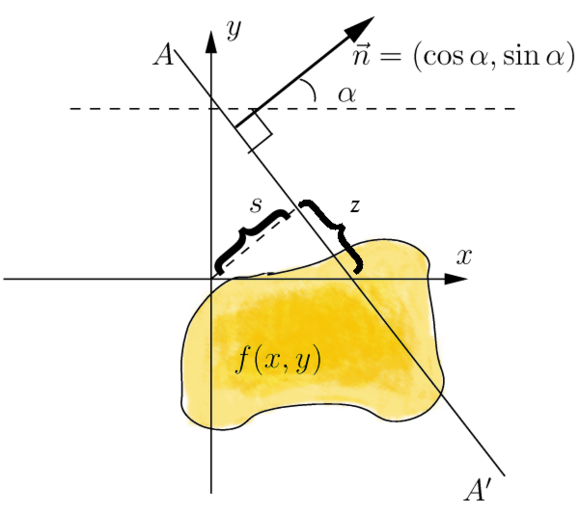
\includegraphics[width=0.55\textwidth]{figures/Radon_transform.png}
\caption{Esquema conceptual de la asignación $f(x,y)\,\rightarrow\,Rf(\alpha,s)$.}
\label{fig:mapping}
\end{figure}
\FloatBarrier

En términos sencillos, la transformada de Radon toma una función
$f(x,y)$ (por ejemplo, la densidad desconocida de un objeto) y genera
otra función $Rf(\alpha,s)$ cuyos valores son integrales de línea de $f$
a lo largo de todas las rectas del plano.  Dicho de otro modo, captura
la “masa” contenida en cada rayo definido por el par $(\alpha,s)$.

\subsection*{Sinogramas}

La representación gráfica de $Rf$ recibe el nombre de
\emph{sinograma}.  Un punto fuera del centro produce una traza
sinusoidal; la superposición de varios objetos se plasma como un bosque
de senos borrosos con distinta fase y amplitud.

\begin{figure}[H]
\centering
\begin{subfigure}[b]{0.47\textwidth}
  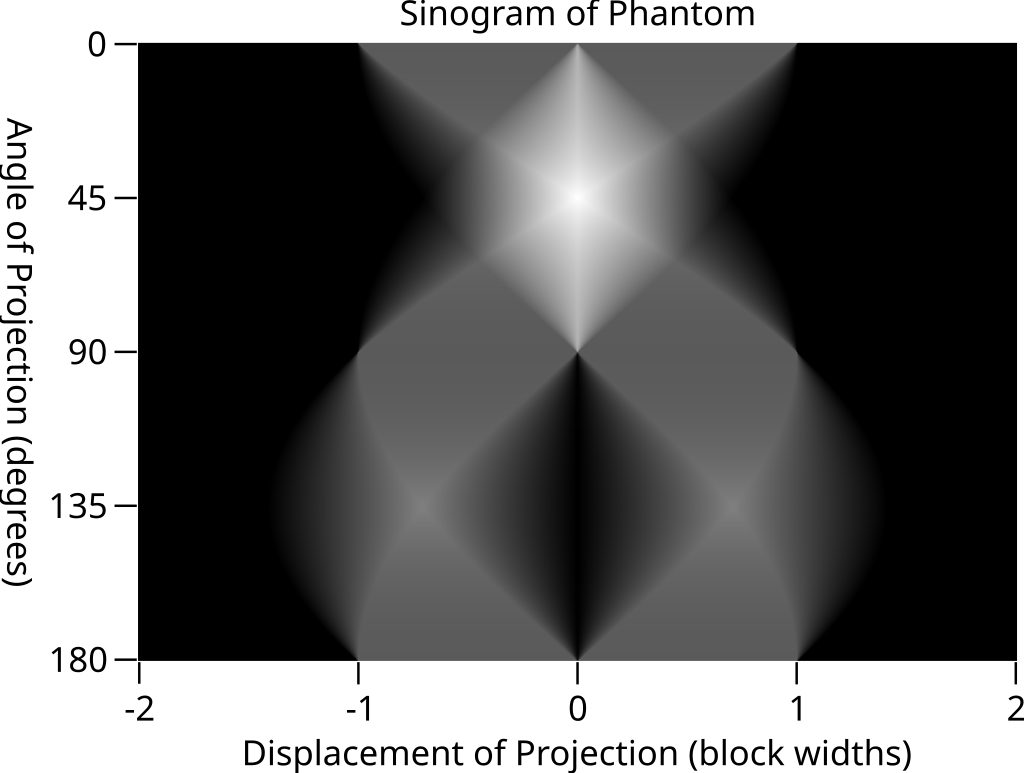
\includegraphics[width=\linewidth]{figures/Sinogram_-_Two_Square_Indicator_Phantom.svg.png}
  \caption{}
\end{subfigure}\hfill
\begin{subfigure}[b]{0.47\textwidth}
  
\includegraphics[width=\linewidth]{figures/Sinogram_Source_-_Two_Squares_Phantom.svg.png}
  \caption{}
\end{subfigure}
\caption{Sinograma obtenido a partir de la función indicadora de dos cuadrados.}
\end{figure}
\FloatBarrier

Las aristas paralelas refuerzan la señal cuando se alinean con la
dirección de proyección, fenómeno que se aprecia claramente en el caso
de los dos cuadrados.

\subsection*{Ámbitos de uso}

La capacidad de reconstruir $f$ a partir de $Rf$ sustenta tecnologías
muy diversas:

\begin{itemize}\itemsep0.3em
\item Tomografía computarizada (CT) y tomografía axial computarizada (CAT)
\item PET y SPECT (medicina nuclear)
\item Microscopía electrónica de partículas (virus, complejos proteicos)
\item Tomografía óptica de proyección
\item Exploración sísmica de reflexión
\item Lectores de códigos de barras y QR (versión 1-D)
\end{itemize}

Todas comparten la misma idea: medir proyecciones desde múltiples
direcciones y luego invertir la transformada para revelar la estructura
interna.

%%%%%%%%%%%%%%%%%%%%%%%%%%%%%%%%%%%%%%%%%%%%%%%%%%%%%%%%%%%%%%%%%%%%%%%%
\section{Experimentos Analíticos}

\subsection{Gaussiana radial}

Con \textit{Symbolic Math Toolbox} se verifica que
$f(x,y)=e^{-(x^{2}+y^{2})}$ tiene transformada independiente de
$\varphi$:
$(\mathcal Rf)(p,\varphi)=\sqrt{\pi}\,e^{-p^{2}}$.

\begin{figure}[H]
\centering
\begin{subfigure}[b]{0.47\textwidth}
  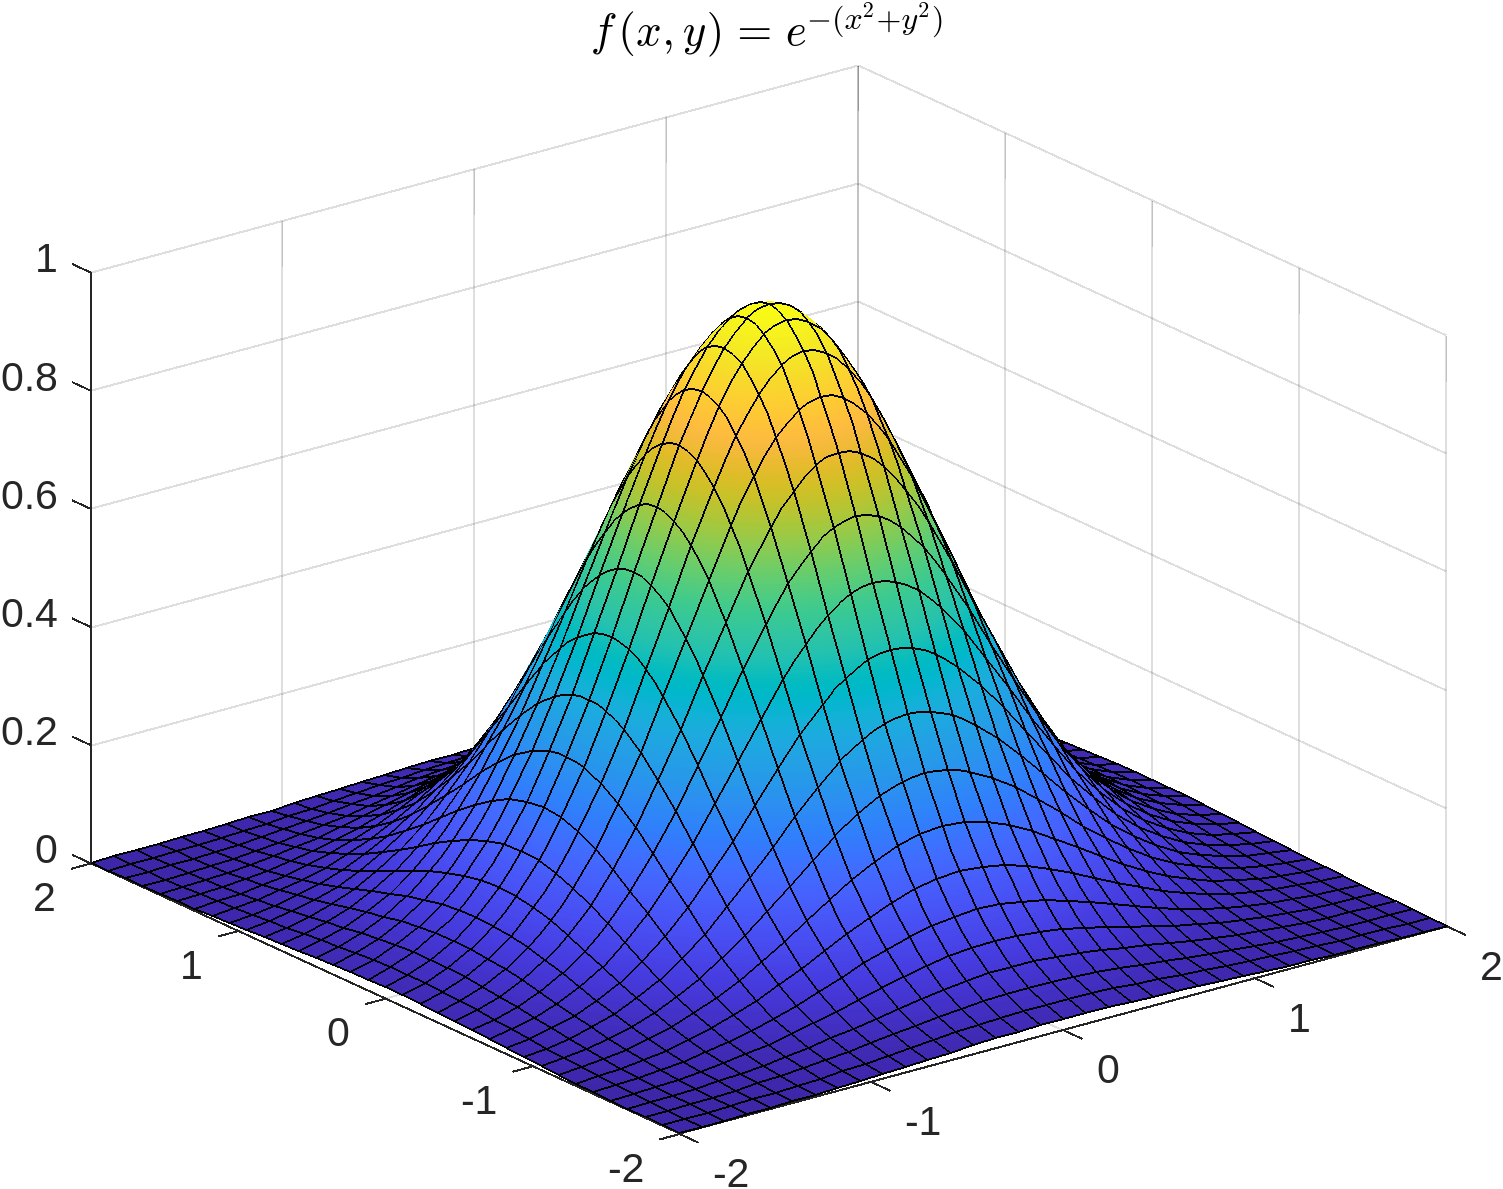
\includegraphics[width=\linewidth]{figures/gaussian_surface.png}
  \caption{Superficie 3-D de $f$.}
\end{subfigure}\hfill
\begin{subfigure}[b]{0.47\textwidth}
  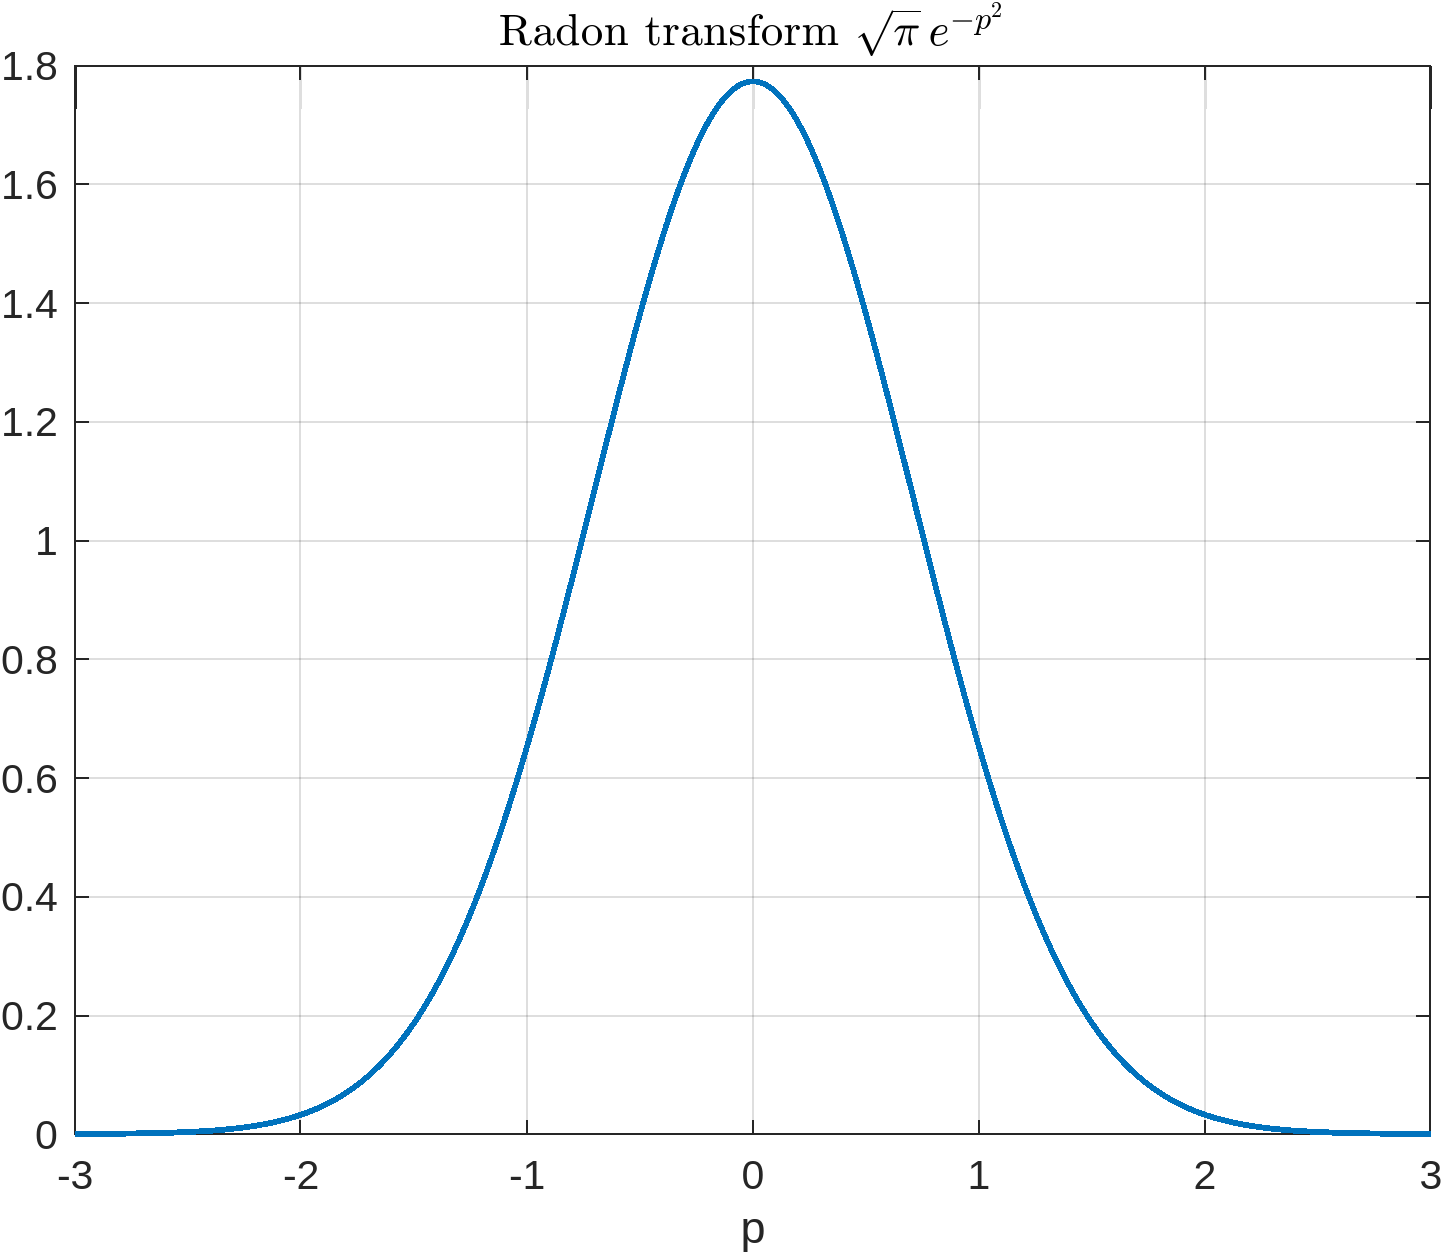
\includegraphics[width=\linewidth]{figures/gaussian_radon.png}
  \caption{$\mathcal Rf$ frente a $p$.}
\end{subfigure}
\caption{Ejemplo radialmente simétrico.}
\label{fig:gaussian}
\end{figure}
\FloatBarrier

\subsection{Polinomio–gaussiana asimétrica}

Para $g(x,y)=(x^{2}+3y^{2})e^{-(x^{2}+y^{2})}$ la simetría radial se
rompe y la transformada depende de $p$ y $\varphi$.

\begin{figure}[H]
\centering
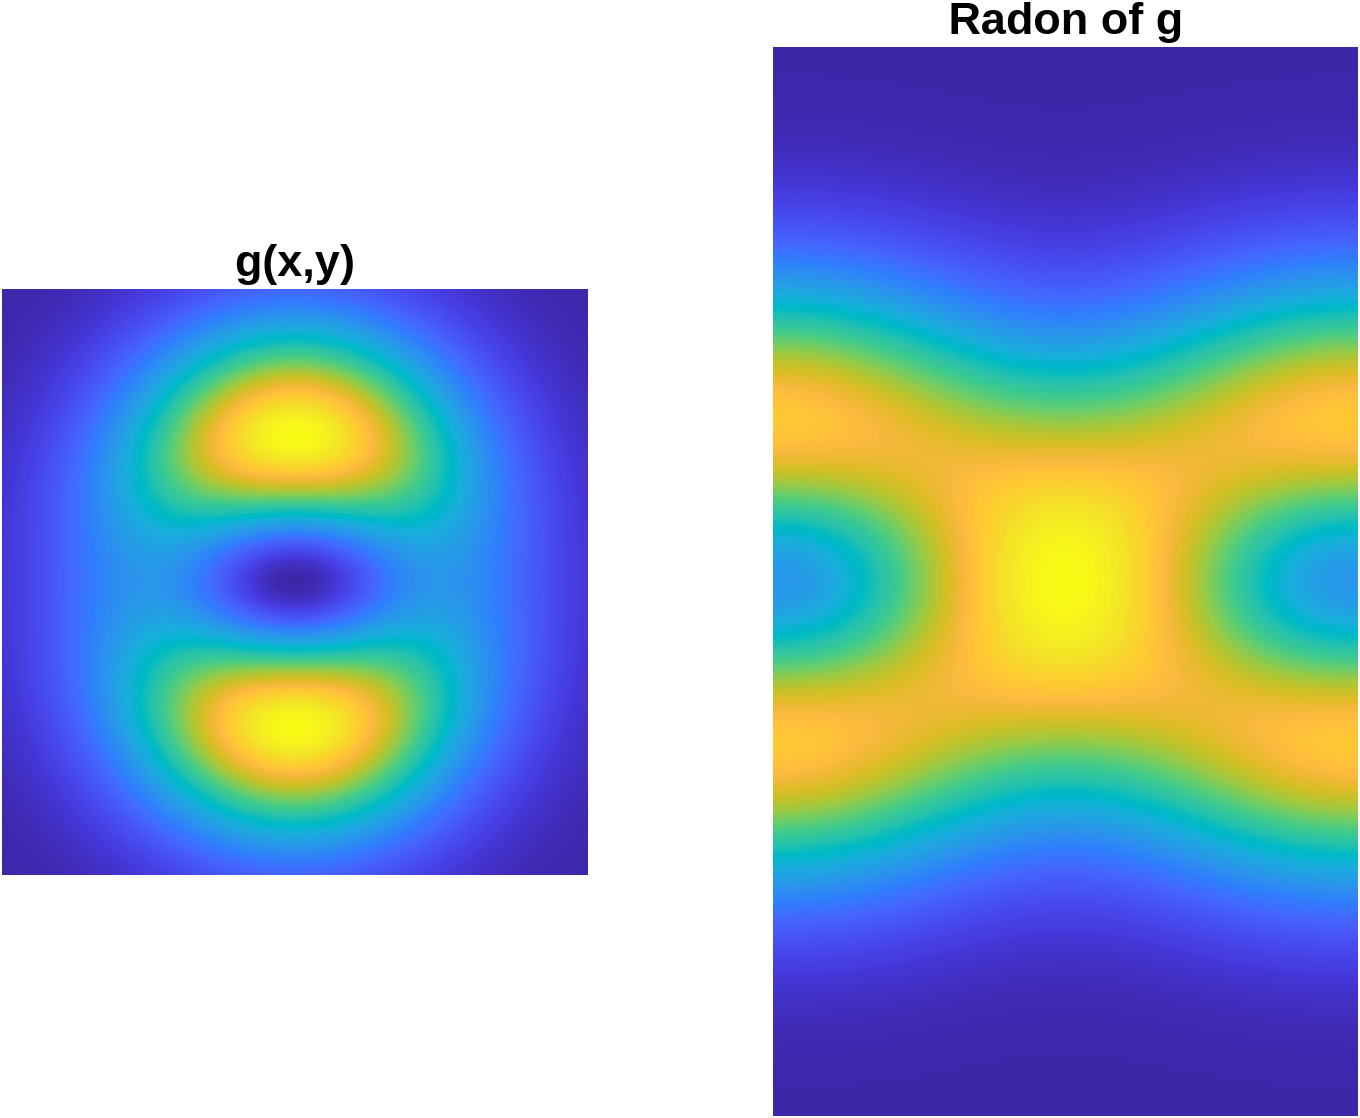
\includegraphics[width=\textwidth]{figures/asymmetric_function_and_radon.png}
\caption{Función asimétrica (izquierda) y su transformada (derecha).}
\label{fig:asymmetric}
\end{figure}
\FloatBarrier

%%%%%%%%%%%%%%%%%%%%%%%%%%%%%%%%%%%%%%%%%%%%%%%%%%%%%%%%%%%%%%%%%%%%%%%%
\section{Experimentos Discretos en MATLAB}

\subsection{Fantoma de disco}

\begin{figure}[H]
\centering
\begin{subfigure}[b]{0.30\textwidth}
  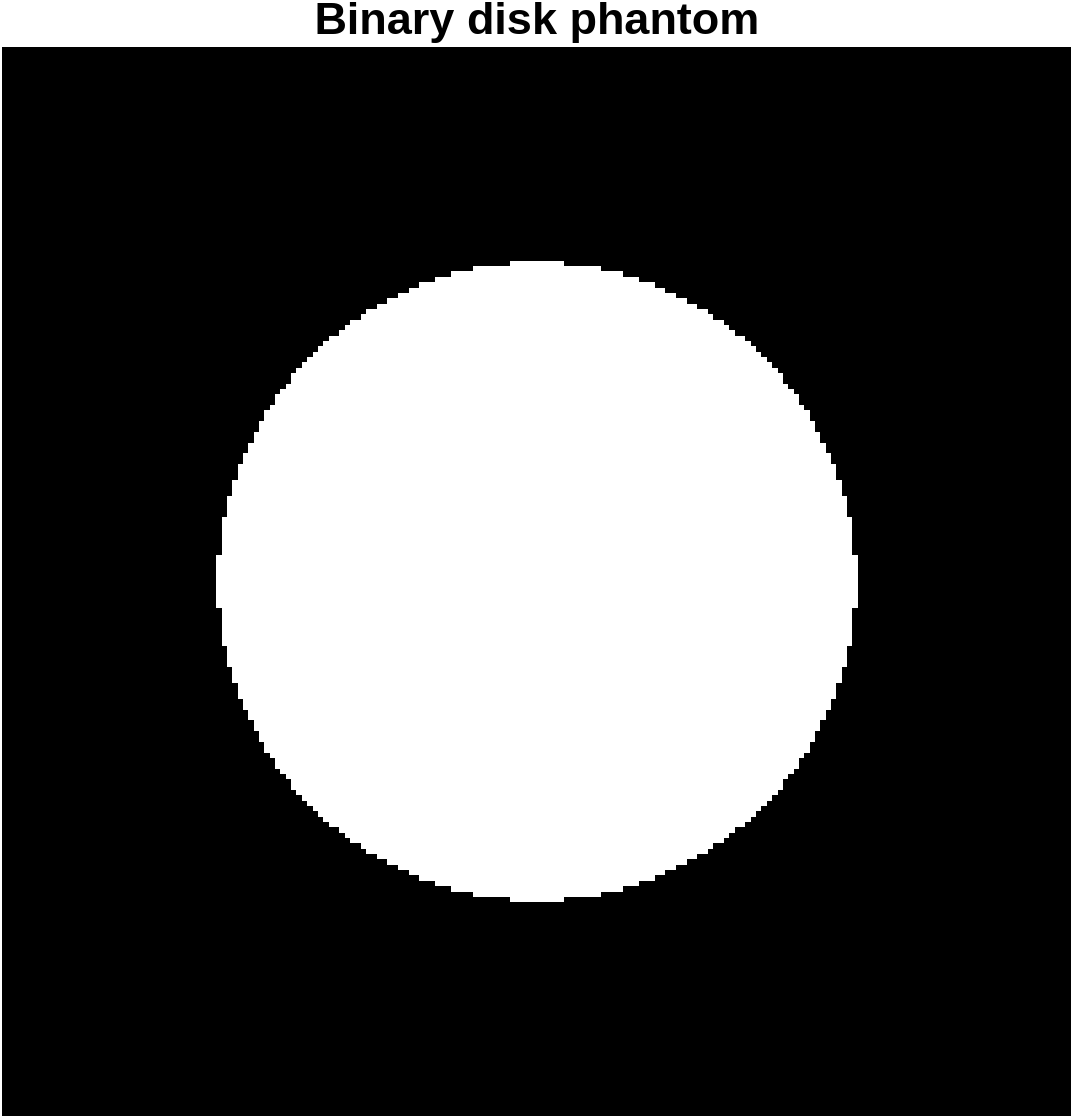
\includegraphics[width=\linewidth]{figures/disk_original.png}
  \caption{Imagen original.}
\end{subfigure}\hfill
\begin{subfigure}[b]{0.34\textwidth}
  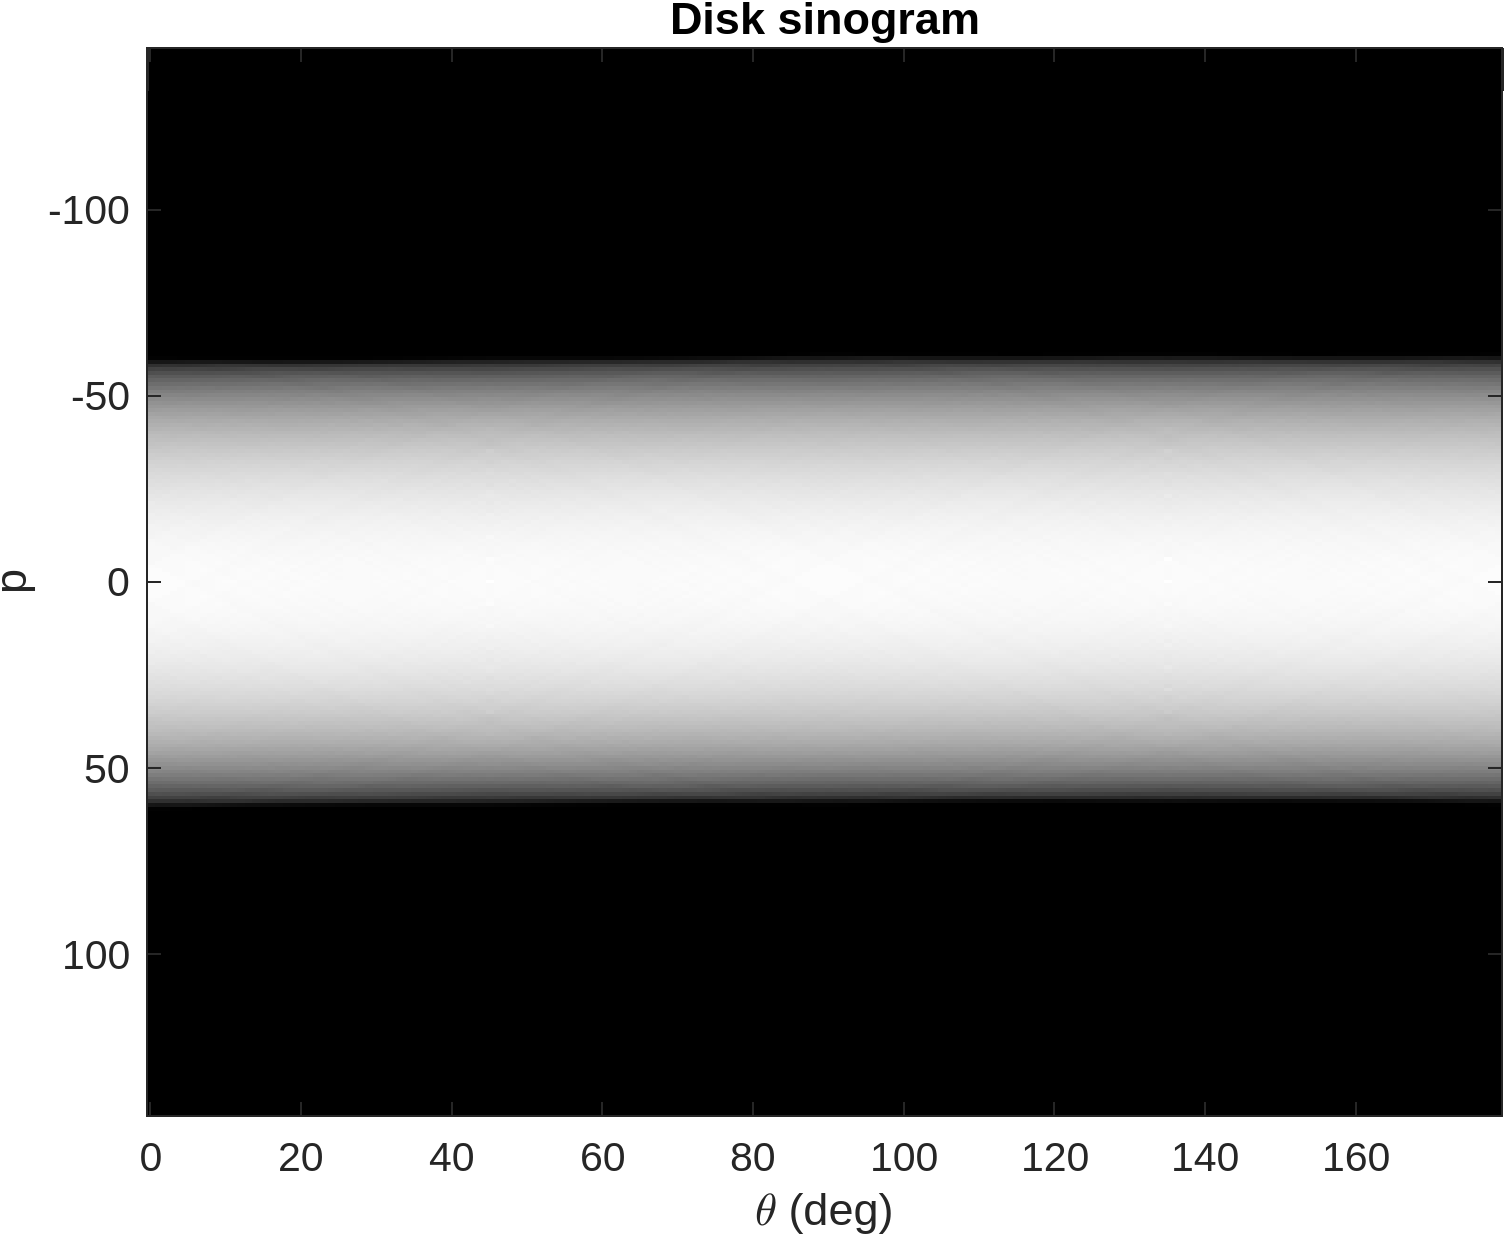
\includegraphics[width=\linewidth]{figures/disk_sinogram.png}
  \caption{Sinograma.}
\end{subfigure}\hfill
\begin{subfigure}[b]{0.30\textwidth}
  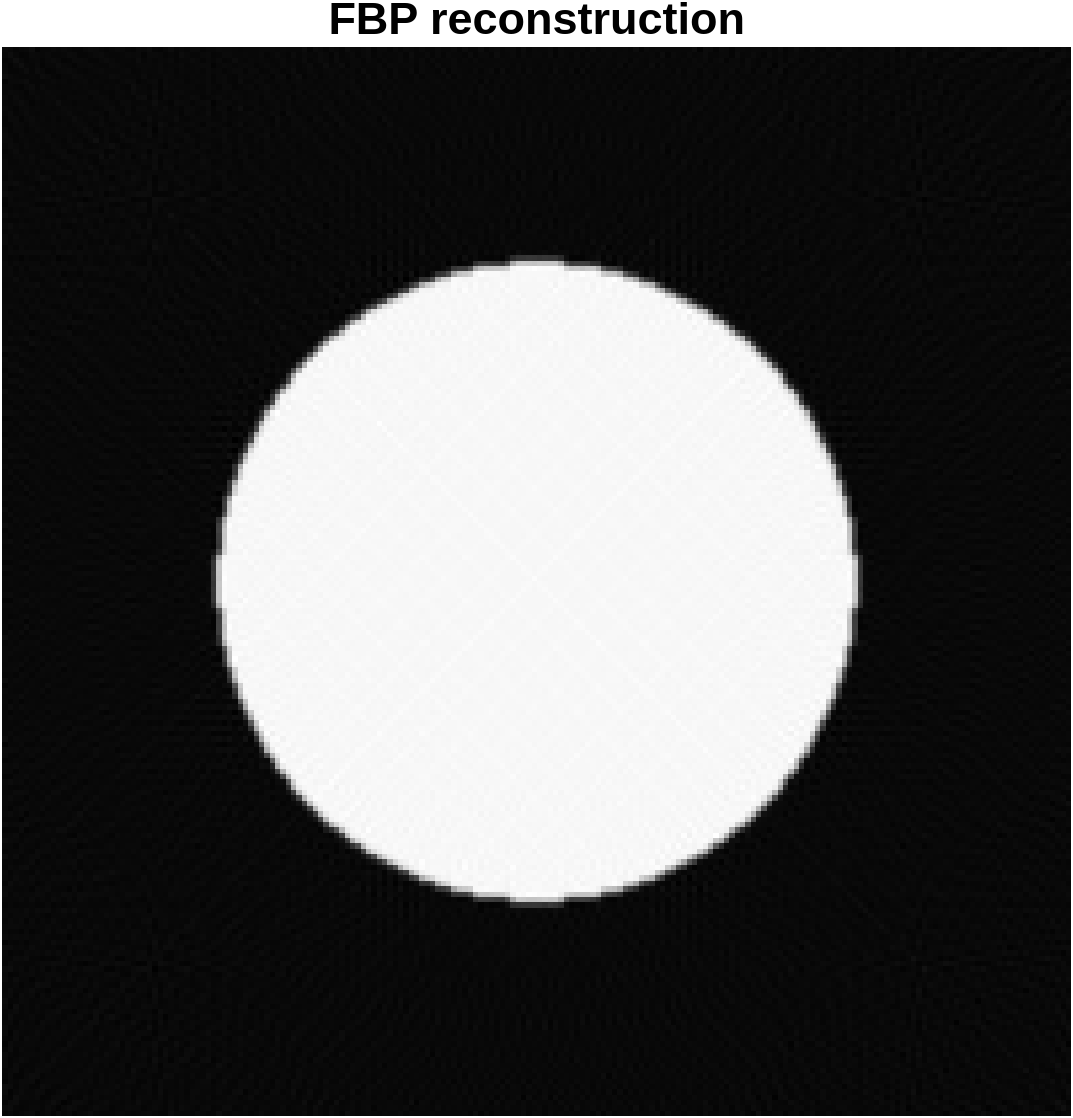
\includegraphics[width=\linewidth]{figures/disk_reconstruction.png}
  \caption{Reconstrucción FBP.}
\end{subfigure}
\caption{Simulación de CT de haz paralelo para un disco.}
\label{fig:disk}
\end{figure}
\FloatBarrier

\subsection{Fantoma de Shepp–Logan}

\begin{figure}[H]
\centering
\begin{subfigure}[b]{0.30\textwidth}
  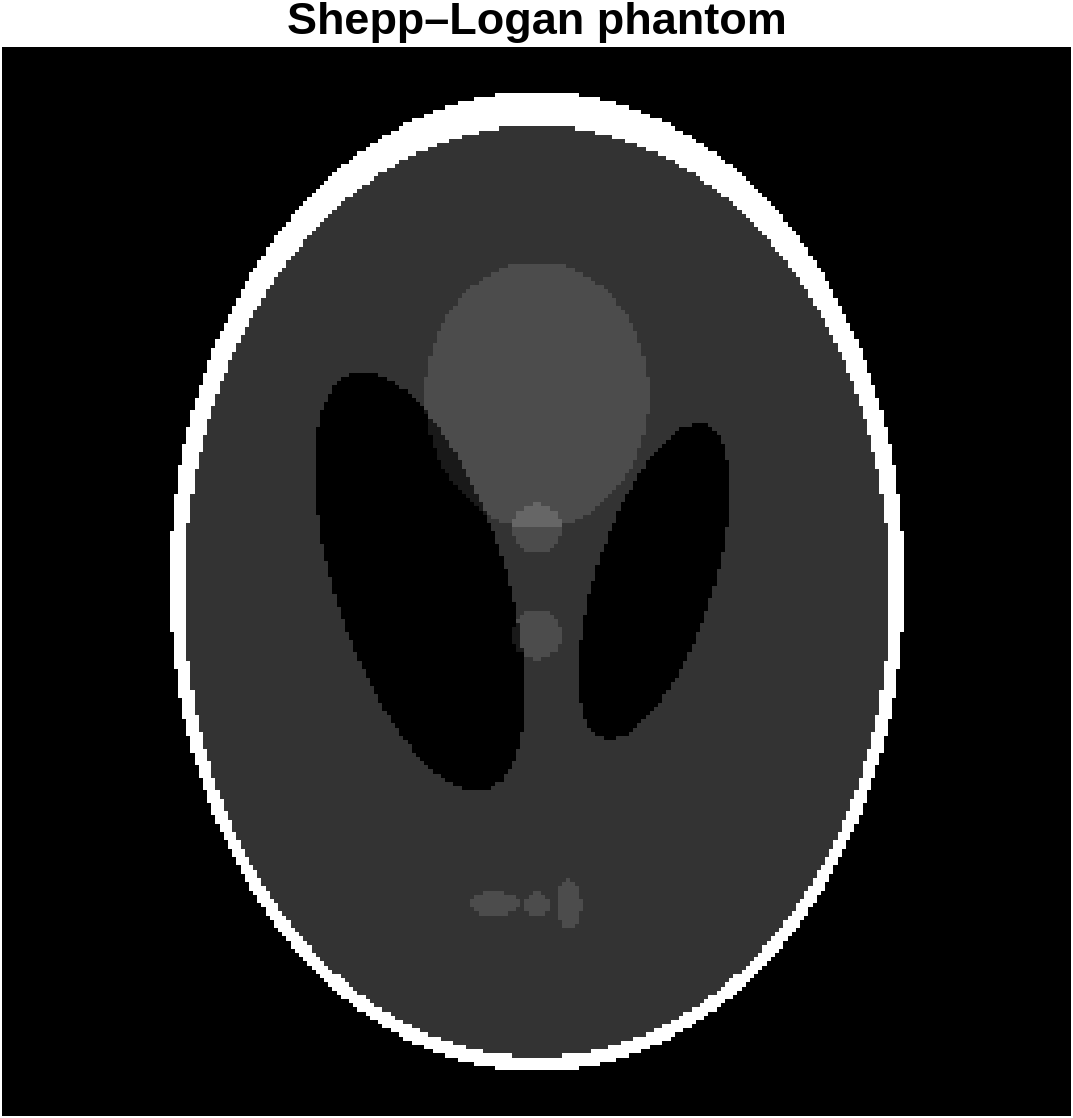
\includegraphics[width=\linewidth]{figures/phantom_original.png}
  \caption{Corte original.}
\end{subfigure}\hfill
\begin{subfigure}[b]{0.34\textwidth}
  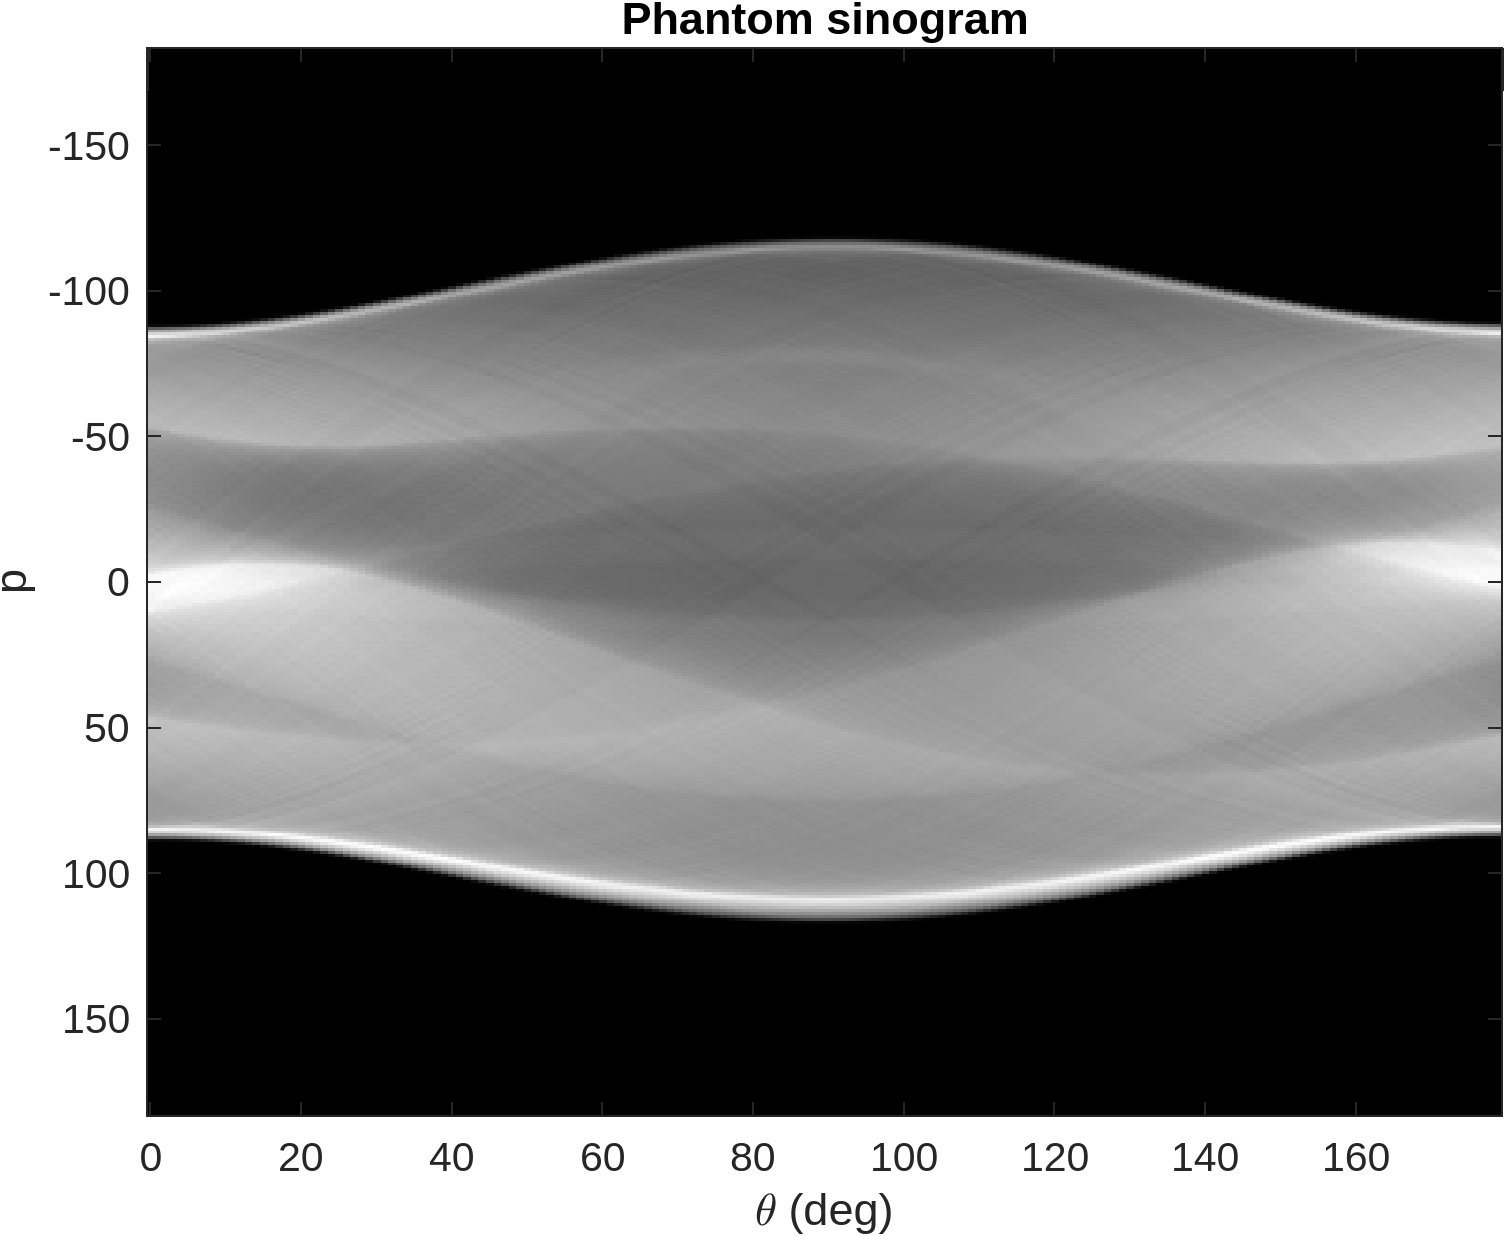
\includegraphics[width=\linewidth]{figures/phantom_sinogram.png}
  \caption{Sinograma.}
\end{subfigure}\hfill
\begin{subfigure}[b]{0.30\textwidth}
  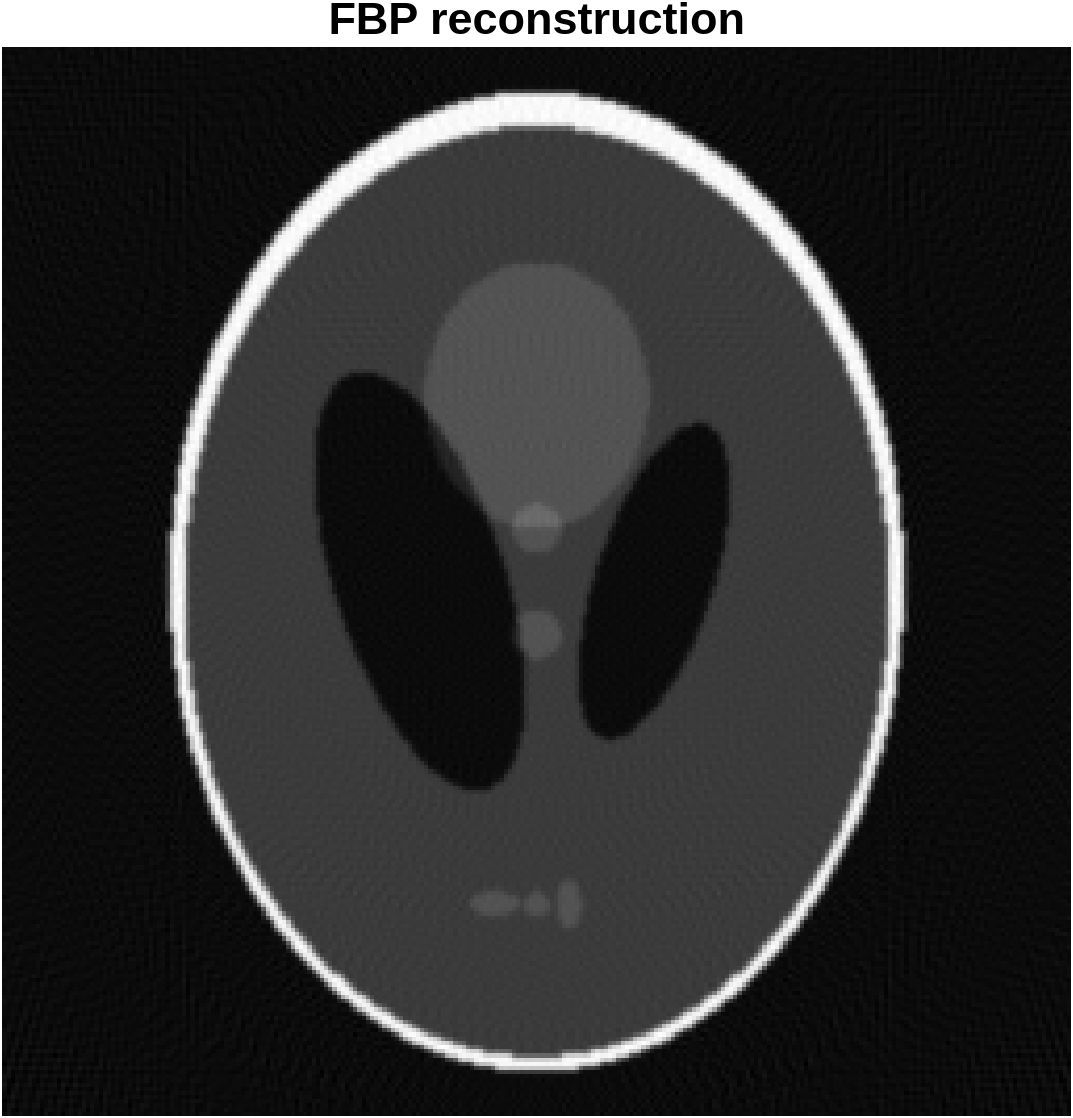
\includegraphics[width=\linewidth]{figures/phantom_reconstruction.png}
  \caption{Reconstrucción.}
\end{subfigure}
\caption{Reconstrucción del fantoma de Shepp–Logan.}
\label{fig:phantom}
\end{figure}
\FloatBarrier

%%%%%%%%%%%%%%%%%%%%%%%%%%%%%%%%%%%%%%%%%%%%%%%%%%%%%%%%%%%%%%%%%%%%%%%%
\section{Contexto en Imagen Biomédica}

\subsection{Del modelo al escáner}

\begin{figure}[H]
\centering
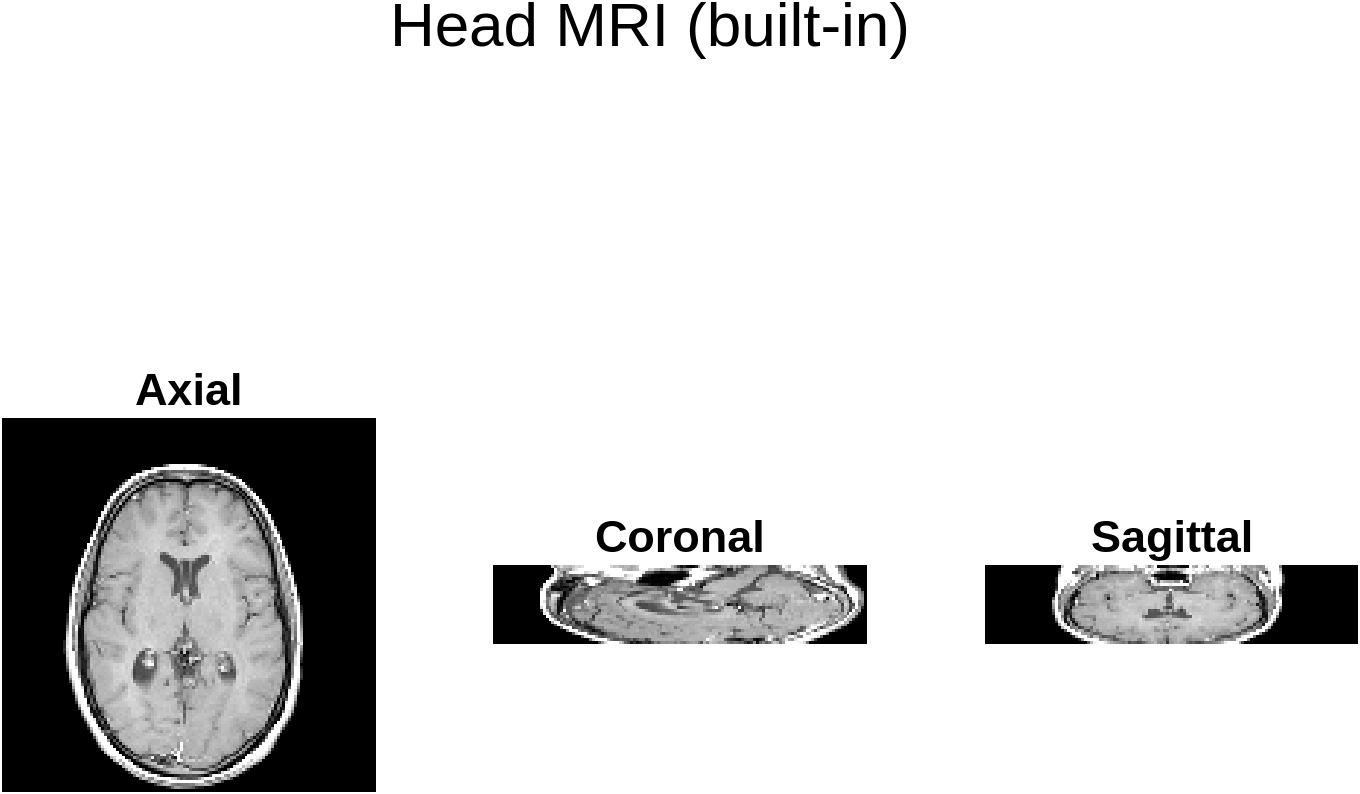
\includegraphics[width=0.68\textwidth]{figures/mri_volume.png}
\caption{Vistas ortogonales de un volumen de ejemplo incluido en MATLAB.}
\label{fig:mri}
\end{figure}
\FloatBarrier

\subsection{Más allá de la CT}

Transformadas tipo Radon también se usan en PET, tomografía óptica,
microscopía electrónica, reflexión sísmica y lectores de códigos de
barras, entre otras aplicaciones.  Investigaciones recientes mezclan
aprendizaje profundo con FBP para reducir la dosis de radiación sin
mermar la calidad diagnóstica.

%%%%%%%%%%%%%%%%%%%%%%%%%%%%%%%%%%%%%%%%%%%%%%%%%%%%%%%%%%%%%%%%%%%%%%%%
\section{Conclusión}

Las pruebas analíticas y numéricas demostraron cómo las integrales de
línea codifican la estructura y cómo la retroproyección filtrada permite
reconstruir imágenes que guían decisiones clínicas.  La transformada de
Radon ejemplifica la sinergia entre geometría, análisis y computación
aplicada a la salud.

%%%%%%%%%%%%%%%%%%%%%%%%%%%%%%%%%%%%%%%%%%%%%%%%%%%%%%%%%%%%%%%%%%%%%%%%
\begin{thebibliography}{9}
\bibitem{Radon1917}
J.~Radon,
\emph{Über die Bestimmung von Funktionen durch ihre Integralwerte
längs gewisser Mannigfaltigkeiten},
\textit{Ber.\ Sächs.\ Akad.\ Wiss.\ Leipzig, Math.-Phys.\ Kl.}
\textbf{69} (1917), 262–277.

\bibitem{CormackHounsfield}
A.~M.~Cormack y G.~N.~Hounsfield,
\emph{Nobel Lectures in Physiology or Medicine 1979},
Nobel Foundation, Estocolmo, 1980.
\end{thebibliography}

\end{document}
